\documentclass{standalone}
\usepackage{tikz}
\usetikzlibrary{patterns, positioning}
\usepackage[sfdefault]{ClearSans} %% option 'sfdefault' activates Clear Sans as the default text font
\usepackage[T1]{fontenc}

\begin{document}
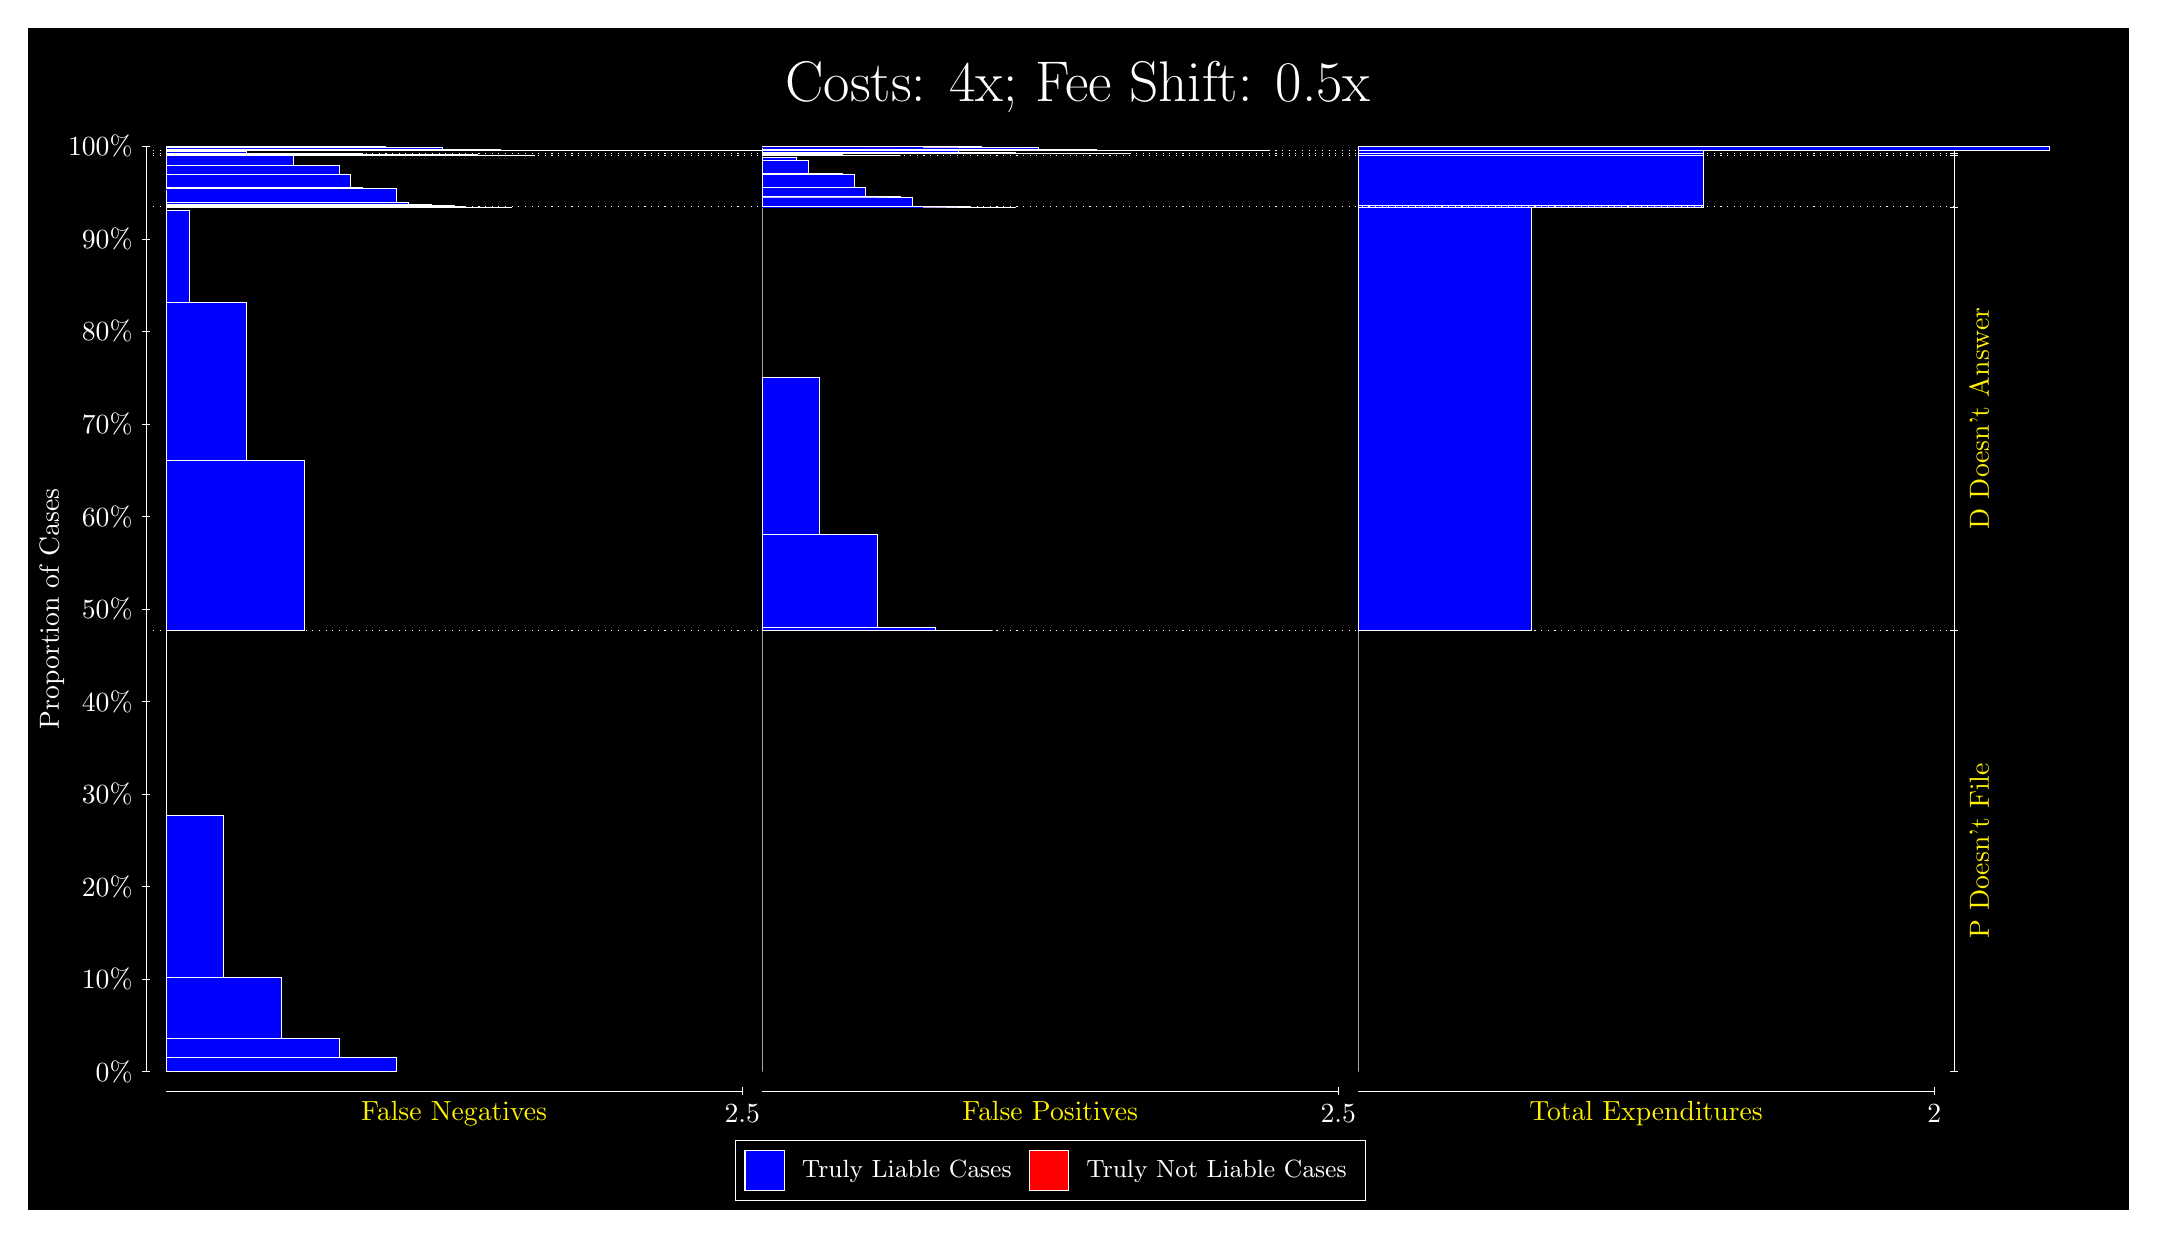
\begin{tikzpicture}
\draw[fill=black] (0,0) rectangle (26.667,15);
\draw[text=white] (0,13.5) rectangle (26.667,15) node[midway] {\huge Costs: 4x; Fee Shift: 0.5x};
\draw[white, very thin] (1.5,1.75) -- (1.5,13.5);
\node[rotate=90, text=white, anchor=center] at (0.3, 7.625) {Proportion of Cases};
\draw[white, very thin] (1.45,1.75) -- (1.55,1.75);
\node[text=white, anchor=east] at (1.45, 1.75) {0\%};
\draw[white, very thin] (1.45,2.925) -- (1.55,2.925);
\node[text=white, anchor=east] at (1.45, 2.925) {10\%};
\draw[white, very thin] (1.45,4.1) -- (1.55,4.1);
\node[text=white, anchor=east] at (1.45, 4.1) {20\%};
\draw[white, very thin] (1.45,5.275) -- (1.55,5.275);
\node[text=white, anchor=east] at (1.45, 5.275) {30\%};
\draw[white, very thin] (1.45,6.45) -- (1.55,6.45);
\node[text=white, anchor=east] at (1.45, 6.45) {40\%};
\draw[white, very thin] (1.45,7.625) -- (1.55,7.625);
\node[text=white, anchor=east] at (1.45, 7.625) {50\%};
\draw[white, very thin] (1.45,8.8) -- (1.55,8.8);
\node[text=white, anchor=east] at (1.45, 8.8) {60\%};
\draw[white, very thin] (1.45,9.975) -- (1.55,9.975);
\node[text=white, anchor=east] at (1.45, 9.975) {70\%};
\draw[white, very thin] (1.45,11.15) -- (1.55,11.15);
\node[text=white, anchor=east] at (1.45, 11.15) {80\%};
\draw[white, very thin] (1.45,12.325) -- (1.55,12.325);
\node[text=white, anchor=east] at (1.45, 12.325) {90\%};
\draw[white, very thin] (1.45,13.5) -- (1.55,13.5);
\node[text=white, anchor=east] at (1.45, 13.5) {100\%};

\draw[white, very thin] (24.457,1.75) -- (24.457,13.5);
\draw[white, very thin] (24.407,1.75) -- (24.507,1.75);
\node[anchor=west] at (24.407, 1.75) {};
\draw[white, very thin] (24.407,7.3532) -- (24.507,7.3532);
\node[anchor=west] at (24.407, 7.3532) {};
\draw[white, very thin] (24.407,12.732) -- (24.507,12.732);
\node[anchor=west] at (24.407, 12.732) {};
\draw[white, very thin] (24.407,13.388) -- (24.507,13.388);
\node[anchor=west] at (24.407, 13.388) {};
\draw[white, very thin] (24.407,13.41) -- (24.507,13.41);
\node[anchor=west] at (24.407, 13.41) {};
\draw[white, very thin] (24.407,13.447) -- (24.507,13.447);
\node[anchor=west] at (24.407, 13.447) {};
\draw[white, very thin] (24.407,13.5) -- (24.507,13.5);
\node[anchor=west] at (24.407, 13.5) {};

\draw[white, very thin, fill=blue] (1.75,1.75) rectangle (4.6775,1.9313);
\draw[white, very thin, fill=blue] (1.75,1.9313) rectangle (3.9457,2.172);
\draw[white, very thin, fill=blue] (1.75,2.172) rectangle (3.2138,2.9438);
\draw[white, very thin, fill=blue] (1.75,2.9438) rectangle (2.4819,5.0061);
\draw[white, very thin, fill=red] (1.75,5.0061) rectangle (1.75,5.0061);
\draw[white, very thin, fill=blue] (1.75,5.0061) rectangle (1.75,7.3532);
\draw[white, very thin, fill=blue] (1.75,7.3532) rectangle (3.5065,9.5131);
\draw[white, very thin, fill=blue] (1.75,9.5131) rectangle (2.7746,11.517);
\draw[white, very thin, fill=blue] (1.75,11.517) rectangle (2.0428,12.691);
\draw[white, very thin, fill=red] (1.75,12.691) rectangle (1.75,12.691);
\draw[white, very thin, fill=blue] (1.75,12.691) rectangle (1.75,12.732);
\draw[white, very thin, fill=blue] (1.75,12.732) rectangle (6.1413,12.732);
\draw[white, very thin, fill=blue] (1.75,12.732) rectangle (5.8486,12.732);
\draw[white, very thin, fill=blue] (1.75,12.732) rectangle (5.5558,12.733);
\draw[white, very thin, fill=blue] (1.75,12.733) rectangle (5.4094,12.756);
\draw[white, very thin, fill=blue] (1.75,12.756) rectangle (5.2631,12.756);
\draw[white, very thin, fill=blue] (1.75,12.756) rectangle (5.1167,12.759);
\draw[white, very thin, fill=blue] (1.75,12.759) rectangle (4.9703,12.765);
\draw[white, very thin, fill=blue] (1.75,12.765) rectangle (4.8239,12.793);
\draw[white, very thin, fill=blue] (1.75,12.793) rectangle (4.6775,12.961);
\draw[white, very thin, fill=blue] (1.75,12.961) rectangle (4.5312,12.962);
\draw[white, very thin, fill=blue] (1.75,12.962) rectangle (4.3848,12.965);
\draw[white, very thin, fill=blue] (1.75,12.965) rectangle (4.2384,12.977);
\draw[white, very thin, fill=blue] (1.75,12.977) rectangle (4.092,13.143);
\draw[white, very thin, fill=blue] (1.75,13.143) rectangle (3.9457,13.26);
\draw[white, very thin, fill=blue] (1.75,13.26) rectangle (3.7993,13.26);
\draw[white, very thin, fill=blue] (1.75,13.26) rectangle (3.6529,13.26);
\draw[white, very thin, fill=blue] (1.75,13.26) rectangle (3.5065,13.263);
\draw[white, very thin, fill=blue] (1.75,13.263) rectangle (3.3602,13.385);
\draw[white, very thin, fill=blue] (1.75,13.385) rectangle (3.2138,13.387);
\draw[white, very thin, fill=blue] (1.75,13.387) rectangle (3.0674,13.387);
\draw[white, very thin, fill=blue] (1.75,13.387) rectangle (2.921,13.387);
\draw[white, very thin, fill=blue] (1.75,13.387) rectangle (2.7746,13.387);
\draw[white, very thin, fill=blue] (1.75,13.387) rectangle (2.6283,13.388);
\draw[white, very thin, fill=blue] (1.75,13.388) rectangle (2.3355,13.388);
\draw[white, very thin, fill=blue] (1.75,13.388) rectangle (2.0428,13.388);
\draw[white, very thin, fill=red] (1.75,13.388) rectangle (1.75,13.388);
\draw[white, very thin, fill=blue] (1.75,13.388) rectangle (6.4341,13.388);
\draw[white, very thin, fill=blue] (1.75,13.388) rectangle (5.7022,13.393);
\draw[white, very thin, fill=blue] (1.75,13.393) rectangle (4.9703,13.404);
\draw[white, very thin, fill=blue] (1.75,13.404) rectangle (4.2384,13.41);
\draw[white, very thin, fill=blue] (1.75,13.41) rectangle (3.5065,13.41);
\draw[white, very thin, fill=red] (1.75,13.41) rectangle (1.75,13.41);
\draw[white, very thin, fill=blue] (1.75,13.41) rectangle (3.5065,13.41);
\draw[white, very thin, fill=blue] (1.75,13.41) rectangle (2.7746,13.431);
\draw[white, very thin, fill=blue] (1.75,13.431) rectangle (2.0428,13.447);
\draw[white, very thin, fill=red] (1.75,13.447) rectangle (1.75,13.447);
\draw[white, very thin, fill=blue] (1.75,13.447) rectangle (1.75,13.447);
\draw[white, very thin, fill=blue] (1.75,13.447) rectangle (9.9471,13.447);
\draw[white, very thin, fill=blue] (1.75,13.447) rectangle (9.2152,13.447);
\draw[white, very thin, fill=blue] (1.75,13.447) rectangle (8.4834,13.448);
\draw[white, very thin, fill=blue] (1.75,13.448) rectangle (7.7515,13.451);
\draw[white, very thin, fill=blue] (1.75,13.451) rectangle (7.4587,13.451);
\draw[white, very thin, fill=blue] (1.75,13.451) rectangle (7.0196,13.451);
\draw[white, very thin, fill=blue] (1.75,13.451) rectangle (6.7268,13.451);
\draw[white, very thin, fill=blue] (1.75,13.451) rectangle (6.2877,13.451);
\draw[white, very thin, fill=blue] (1.75,13.451) rectangle (5.9949,13.461);
\draw[white, very thin, fill=blue] (1.75,13.461) rectangle (5.2631,13.487);
\draw[white, very thin, fill=blue] (1.75,13.487) rectangle (4.5312,13.499);
\draw[white, very thin, fill=blue] (1.75,13.499) rectangle (3.7993,13.5);
\draw[white, very thin, fill=blue] (1.75,13.5) rectangle (3.0674,13.5);
\draw[white, very thin, fill=blue] (1.75,13.5) rectangle (2.3355,13.5);
\draw[white, very thin, fill=red] (1.75,13.5) rectangle (1.75,13.5);
\draw[white, very thin, fill=red] (9.3189,1.75) rectangle (9.3189,1.75);
\draw[white, very thin, fill=blue] (9.3189,1.75) rectangle (9.3189,7.3532);
\draw[white, very thin, fill=red] (9.3189,7.3532) rectangle (12.246,7.3532);
\draw[white, very thin, fill=blue] (9.3189,7.3532) rectangle (12.246,7.3532);
\draw[white, very thin, fill=blue] (9.3189,7.3532) rectangle (11.515,7.3939);
\draw[white, very thin, fill=blue] (9.3189,7.3939) rectangle (10.783,8.5684);
\draw[white, very thin, fill=blue] (9.3189,8.5684) rectangle (10.051,10.572);
\draw[white, very thin, fill=blue] (9.3189,10.572) rectangle (9.3189,12.732);
\draw[white, very thin, fill=red] (9.3189,12.732) rectangle (12.539,12.732);
\draw[white, very thin, fill=blue] (9.3189,12.732) rectangle (12.539,12.732);
\draw[white, very thin, fill=red] (9.3189,12.732) rectangle (12.246,12.732);
\draw[white, very thin, fill=blue] (9.3189,12.732) rectangle (12.246,12.732);
\draw[white, very thin, fill=red] (9.3189,12.732) rectangle (11.954,12.732);
\draw[white, very thin, fill=blue] (9.3189,12.732) rectangle (11.954,12.733);
\draw[white, very thin, fill=blue] (9.3189,12.733) rectangle (11.807,12.733);
\draw[white, very thin, fill=red] (9.3189,12.733) rectangle (11.661,12.733);
\draw[white, very thin, fill=blue] (9.3189,12.733) rectangle (11.661,12.733);
\draw[white, very thin, fill=blue] (9.3189,12.733) rectangle (11.515,12.733);
\draw[white, very thin, fill=red] (9.3189,12.733) rectangle (11.368,12.733);
\draw[white, very thin, fill=blue] (9.3189,12.733) rectangle (11.368,12.735);
\draw[white, very thin, fill=blue] (9.3189,12.735) rectangle (11.222,12.857);
\draw[white, very thin, fill=blue] (9.3189,12.857) rectangle (11.075,12.86);
\draw[white, very thin, fill=blue] (9.3189,12.86) rectangle (10.929,12.86);
\draw[white, very thin, fill=blue] (9.3189,12.86) rectangle (10.783,12.86);
\draw[white, very thin, fill=blue] (9.3189,12.86) rectangle (10.636,12.977);
\draw[white, very thin, fill=blue] (9.3189,12.977) rectangle (10.49,13.143);
\draw[white, very thin, fill=blue] (9.3189,13.143) rectangle (10.344,13.155);
\draw[white, very thin, fill=blue] (9.3189,13.155) rectangle (10.197,13.158);
\draw[white, very thin, fill=blue] (9.3189,13.158) rectangle (10.051,13.159);
\draw[white, very thin, fill=blue] (9.3189,13.159) rectangle (9.9044,13.327);
\draw[white, very thin, fill=blue] (9.3189,13.327) rectangle (9.758,13.355);
\draw[white, very thin, fill=blue] (9.3189,13.355) rectangle (9.6116,13.361);
\draw[white, very thin, fill=blue] (9.3189,13.361) rectangle (9.4652,13.364);
\draw[white, very thin, fill=blue] (9.3189,13.364) rectangle (9.3189,13.388);
\draw[white, very thin, fill=red] (9.3189,13.388) rectangle (11.075,13.388);
\draw[white, very thin, fill=blue] (9.3189,13.388) rectangle (11.075,13.388);
\draw[white, very thin, fill=blue] (9.3189,13.388) rectangle (10.344,13.394);
\draw[white, very thin, fill=blue] (9.3189,13.394) rectangle (9.6116,13.405);
\draw[white, very thin, fill=blue] (9.3189,13.405) rectangle (9.3189,13.41);
\draw[white, very thin, fill=red] (9.3189,13.41) rectangle (14.003,13.41);
\draw[white, very thin, fill=blue] (9.3189,13.41) rectangle (14.003,13.41);
\draw[white, very thin, fill=blue] (9.3189,13.41) rectangle (13.271,13.41);
\draw[white, very thin, fill=blue] (9.3189,13.41) rectangle (12.539,13.427);
\draw[white, very thin, fill=blue] (9.3189,13.427) rectangle (11.807,13.447);
\draw[white, very thin, fill=blue] (9.3189,13.447) rectangle (11.075,13.447);
\draw[white, very thin, fill=red] (9.3189,13.447) rectangle (15.759,13.447);
\draw[white, very thin, fill=blue] (9.3189,13.447) rectangle (15.759,13.447);
\draw[white, very thin, fill=blue] (9.3189,13.447) rectangle (15.028,13.447);
\draw[white, very thin, fill=red] (9.3189,13.447) rectangle (15.028,13.447);
\draw[white, very thin, fill=blue] (9.3189,13.447) rectangle (15.028,13.447);
\draw[white, very thin, fill=blue] (9.3189,13.447) rectangle (14.296,13.448);
\draw[white, very thin, fill=red] (9.3189,13.448) rectangle (14.296,13.448);
\draw[white, very thin, fill=blue] (9.3189,13.448) rectangle (14.296,13.448);
\draw[white, very thin, fill=blue] (9.3189,13.448) rectangle (13.564,13.451);
\draw[white, very thin, fill=red] (9.3189,13.451) rectangle (13.564,13.451);
\draw[white, very thin, fill=blue] (9.3189,13.451) rectangle (13.564,13.46);
\draw[white, very thin, fill=blue] (9.3189,13.46) rectangle (12.832,13.461);
\draw[white, very thin, fill=blue] (9.3189,13.461) rectangle (12.832,13.486);
\draw[white, very thin, fill=blue] (9.3189,13.486) rectangle (12.1,13.496);
\draw[white, very thin, fill=red] (9.3189,13.496) rectangle (11.807,13.496);
\draw[white, very thin, fill=blue] (9.3189,13.496) rectangle (11.807,13.496);
\draw[white, very thin, fill=blue] (9.3189,13.496) rectangle (11.368,13.497);
\draw[white, very thin, fill=red] (9.3189,13.497) rectangle (11.075,13.497);
\draw[white, very thin, fill=blue] (9.3189,13.497) rectangle (11.075,13.497);
\draw[white, very thin, fill=blue] (9.3189,13.497) rectangle (10.636,13.497);
\draw[white, very thin, fill=blue] (9.3189,13.497) rectangle (10.344,13.499);
\draw[white, very thin, fill=blue] (9.3189,13.499) rectangle (9.6116,13.5);
\draw[white, very thin, fill=blue] (9.3189,13.5) rectangle (9.3189,13.5);
\draw[white, very thin, fill=red] (16.888,1.75) rectangle (16.888,1.75);
\draw[white, very thin, fill=blue] (16.888,1.75) rectangle (16.888,7.3532);
\draw[white, very thin, fill=red] (16.888,7.3532) rectangle (19.083,7.3532);
\draw[white, very thin, fill=blue] (16.888,7.3532) rectangle (19.083,12.732);
\draw[white, very thin, fill=red] (16.888,12.732) rectangle (21.279,12.732);
\draw[white, very thin, fill=blue] (16.888,12.732) rectangle (21.279,12.753);
\draw[white, very thin, fill=red] (16.888,12.753) rectangle (21.279,12.753);
\draw[white, very thin, fill=blue] (16.888,12.753) rectangle (21.279,13.388);
\draw[white, very thin, fill=red] (16.888,13.388) rectangle (21.279,13.388);
\draw[white, very thin, fill=blue] (16.888,13.388) rectangle (21.279,13.41);
\draw[white, very thin, fill=red] (16.888,13.41) rectangle (21.279,13.41);
\draw[white, very thin, fill=blue] (16.888,13.41) rectangle (21.279,13.447);
\draw[white, very thin, fill=red] (16.888,13.447) rectangle (25.67,13.447);
\draw[white, very thin, fill=blue] (16.888,13.447) rectangle (25.67,13.452);
\draw[white, very thin, fill=red] (16.888,13.452) rectangle (25.67,13.452);
\draw[white, very thin, fill=blue] (16.888,13.452) rectangle (25.67,13.5);
\draw[white, dotted] (1.5,7.3532) -- (24.457,7.3532);
\draw[white, dotted] (1.5,12.732) -- (24.457,12.732);
\draw[white, dotted] (1.5,13.388) -- (24.457,13.388);
\draw[white, dotted] (1.5,13.41) -- (24.457,13.41);
\draw[white, dotted] (1.5,13.447) -- (24.457,13.447);
\draw[white, very thin] (1.75,1.5) -- (9.0689,1.5);
\node[text=yellow, anchor=north] at (5.4094, 1.5) {False Negatives};
\draw[white, very thin] (9.0689,1.45) -- (9.0689,1.55);
\node[text=white, anchor=north] at (9.0689, 1.45) {2.5};

\draw[white, very thin] (9.3189,1.5) -- (16.638,1.5);
\node[text=yellow, anchor=north] at (12.978, 1.5) {False Positives};
\draw[white, very thin] (16.638,1.45) -- (16.638,1.55);
\node[text=white, anchor=north] at (16.638, 1.45) {2.5};

\draw[white, very thin] (16.888,1.5) -- (24.207,1.5);
\node[text=yellow, anchor=north] at (20.547, 1.5) {Total Expenditures};
\draw[white, very thin] (24.207,1.45) -- (24.207,1.55);
\node[text=white, anchor=north] at (24.207, 1.45) {2};

\node[text=yellow, centered, rotate=90] at (24.777, 4.5516) {P Doesn't File};
\node[text=yellow, centered, rotate=90] at (24.777, 10.043) {D Doesn't Answer};





\draw (12.978300999999998,1.5) node[draw=none] (baseCoordinate) {};
\begin{scope}[align=center]
        \matrix[scale=0.5, draw=white, below=0.5cm of baseCoordinate, nodes={draw}, column sep=0.1cm]{
            \node[rectangle, draw, minimum width=0.5cm, minimum height=0.5cm, fill=blue] {}; &
            \node[draw=none, font=\small, text=white] (B) {Truly Liable Cases}; &
            \node[rectangle, draw, minimum width=0.5cm, minimum height=0.5cm, fill=red] {}; &
            \node[draw=none, font=\small, text=white] (B) {Truly Not Liable Cases}; \\
            };
\end{scope}

\end{tikzpicture}
\end{document}